% SenseEdge rev. A silicon test plan.  Build: tectonic plan/test_plan.tex
\documentclass[10pt]{article}
\usepackage[margin=0.9in]{geometry}
\usepackage{booktabs,array,longtable,tabularx}
\usepackage{amsmath}
\usepackage{siunitx}
\usepackage{enumitem}
\usepackage{xcolor}
\usepackage{tikz}
\usetikzlibrary{arrows.meta,positioning}
\usepackage[colorlinks=true,linkcolor=blue!50!black,urlcolor=blue!50!black]{hyperref}

\newcolumntype{L}[1]{>{\raggedright\arraybackslash}p{#1}}
\newcommand{\tid}[1]{\textbf{#1}}
\newcommand{\pred}[1]{\textit{#1}}
\setlist{leftmargin=1.4em,itemsep=1pt,topsep=3pt}
\setlength{\LTpre}{6pt}\setlength{\LTpost}{8pt}
\renewcommand{\arraystretch}{1.12}

\title{\textbf{SenseEdge Rev.~A Silicon Test Plan}\\[2pt]
\large Measurements for the CICC $\rightarrow$ JSSC paper}
\author{Fidel Makatia Omusilibwa}
\date{October 2026 \quad(companion to \texttt{plan/plan.tex} and \texttt{paper/main.tex})}

\begin{document}
\maketitle

\section*{Bottom line}
\noindent\fbox{\parbox{0.975\linewidth}{\small
\textbf{What revision A can prove, to journal standard.}
(1)~Acquisition, FFT, and feature extraction that match the RTL bit for bit
across supply, frequency, temperature, and at least 20 dice.
(2)~Energy: per clock, per classification window, minimum-energy point,
leakage, and a phase-resolved breakdown.
(3)~A same-die comparison of the hardware pipeline against the same
pipeline in software on the Caravel RISC-V core.
(4)~Signal-chain fidelity against reference instrumentation.
(5)~Accuracy and a multi-week deployment on physical faults, with the
features computed in hardware and the classifier in firmware on the same
die.

\textbf{What it cannot prove.} The on-chip network cannot be programmed:
22 of its 212 weights are writable and the rest hold their power-up
state. A search over the 22 writable weights does not rescue it. In
simulation over 40 random power-up states, on a task that a fully
loadable network solves at \SI{100}{\percent}, the median accuracy after
the search is \SI{37}{\percent} and no state reaches \SI{90}{\percent}.
The claims ``no processor in the inference loop'' and ``in-field model
update through the register map'' therefore cannot be measured on this
silicon.

\textbf{The operating point that matters.} The clock is not gated, so
energy per classification is set by the number of clocks per window,
$2240\,(D+1)$ for divider $D\ge1$ and \num{2304} at $D=0$. At the reset
divider and \SI{20}{\mega\hertz} that is \SI{0.36}{\milli\joule}. With
$D=0$ and the clock set to 36 times the sample rate it is predicted at
\SI{1.5}{\micro\joule}, with an average macro power of
\SI{54}{\micro\watt} at \SI{2.29}{kS/s}. RTL simulation gives identical
FFT bins and features at $D=0$. The campaign is built around measuring
this point.

\textbf{Decision needed now (gate G0).} Either the paper is reframed
around what revision A measures, or the JSSC version waits for a
corrected revision B. Section~\ref{sec:claims} lists every claim in the
draft that changes.}}

\section{Claims in the draft against what can be measured}
\label{sec:claims}
Each row is a statement in \texttt{paper/main.tex}. ``Tests'' refers to
Section~\ref{sec:tests}.

{\small
\begin{longtable}{@{}L{4.5cm}L{4.3cm}L{1.6cm}L{4.6cm}@{}}
\toprule
Claim in the draft & Status on revision A & Tests & Action\\
\midrule
\endhead
Acquisition, FFT, features, classification, and alarm ``entirely in
hardware'' & Acquisition, FFT, features: yes. Classification and alarm:
the network runs but its weights are not programmable & B1--B5, N1 &
State where the classifier runs. Hardware classifier is a revision~B
result\\\addlinespace[2pt]
``\textit{X}~\si{\micro\joule} per classification at \textit{X}~MHz,
\textit{X}~V'' & Measurable. The network executes on every window, so its
energy is included & C2, C4, C5 & Define a classification as one
64-sample window; report $D$ and $f_{\mathrm{clk}}$ with every number\\\addlinespace[2pt]
``Duty-cycled average node power at one classification per second'' &
No on-chip gating. Duty cycling means stopping or slowing the external
clock & C4, E3 & Report clock policy. Node board needs a controllable
clock source (Appendix~\ref{app:board})\\\addlinespace[2pt]
``\textit{XX.X}\% accuracy on four physical fault classes,
\textit{X}-week deployment'' & Measurable with hardware features and the
classifier in firmware & F1--F5 & Report as hybrid; give the ladder of
F3 so the cost of the front end is visible\\\addlinespace[2pt]
``In-field model updates through a register-mapped weight interface'' &
Not on revision A & N1 & Firmware-table update only; register-map update
moves to revision B\\\addlinespace[2pt]
``Samples a 12-bit ADC at up to \SI{100}{kS/s}'' & ADC serial-clock
rating limits the rate; expect about \SI{44}{kS/s} at \SI{3.3}{\volt} &
D1 & Replace with the measured maximum\\\addlinespace[2pt]
``One acquisition-to-alarm pass takes \num{11924} cycles'';
``latency \SI{596}{\micro\second}'' & \num{11924} is one window at
$D=4$ in simulation. Buffer-full to decision is 729 clocks & B4 &
Replace: 729 clocks (\SI{36.5}{\micro\second} at \SI{20}{\mega\hertz});
window $2240\,(D+1)$ clocks, \num{2304} at $D=0$\\\addlinespace[2pt]
``Closing timing at \SI{20}{\mega\hertz}'' & Register-to-register slack
$+$\SI{7.0}{\nano\second} at the slow corner; port paths violate on
paper & C3 & Report measured $f_{\max}$ and the port-path caveat\\\addlinespace[2pt]
``Bit-exact FFT/NN cross-checks against Python references \ldots
gate-level simulation with SDF'' & The earlier network reference was not
bit-exact; gate-level runs are functional, not SDF & B2, B3 & Cite the
netlist-accurate reference and the post-route equivalence run\\\addlinespace[2pt]
Energy decomposition ``using per-block enables'' & There is one enable.
Blocks run in sequence & C6 & Decompose by time-resolved current\\\addlinespace[2pt]
``$\sim$50$\times$ frequency and \textit{X}$\times$ energy step'' to
7\,nm & Needs the measured \SI{130}{\nano\metre} energy with the same
definition of a classification & C5 & Fill after C5; state both
operating points\\
\bottomrule
\end{longtable}}

\section{Pre-silicon predictions to be correlated}
\label{sec:pred}
Every measurement is compared with a number fixed before silicon. The
predictions come from RTL and post-route simulation and from the final
hardening run (\texttt{proposal/data/}). A model-to-hardware table built
from this list goes in the paper (test C9).

{\small
\begin{longtable}{@{}L{5.2cm}L{5.6cm}L{4.2cm}@{}}
\toprule
Quantity & Prediction & Test\\
\midrule
\endhead
Buffer full to decision & 729 clocks: FFT 483, features 37, network 209 & B4\\
Clocks per window & $2240\,(D+1)$ for $D\ge1$; \num{2304} at $D=0$ (36 per sample) & B4\\
Sample rate & $f_s=f_{\mathrm{clk}}/[35\,(D+1)]$ for $D\ge1$; $f_{\mathrm{clk}}/36$ at $D=0$ & B4, D1\\
Capture & $2\,(c-2048)+c_1$ within $\pm1024$ codes; wraps outside & B1\\
Bands as computed & bins 2--5, 6--11, 12--21, 22--31 plus DC; peak one bin low & B3\\
Weight registers reachable & 22 of 212 & N1\\
Macro power, \SI{20}{\mega\hertz}, \SI{1.8}{\volt}, \SI{25}{\celsius} &
\SI{12.9}{\milli\watt} (\SI{7.2}{\milli\ampere} on \texttt{vccd2}); 10.5 to \SI{15.0}{\milli\watt} over corners & C2\\
Energy per clock, \SI{1.8}{\volt} & \SI{0.65}{\nano\joule}; \SI{88}{\percent} clock network and flip-flop clock pins & C2, C6\\
Leakage & \SI{0.7}{\micro\watt} typical at \SI{25}{\celsius}; \SI{0.34}{\milli\watt} slow corner at \SI{100}{\celsius} & C1\\
Energy per classification & \SI{1.5}{\micro\joule} at $D=0$; \SI{0.36}{\milli\joule} at reset; \SI{0.47}{\micro\joule} for the 729-clock pass alone & C4, C5\\
Longest register-to-register path & \SI{22.1}{\nano\second} typical, \SI{41.8}{\nano\second} slow: $f_{\max}\approx$ \SI{42}{\mega\hertz} typical, \SI{23}{\mega\hertz} slow & C3\\
Hold margin, register to register & $+$\SI{0.06}{\nano\second} at the fast corner & C3 (hold signature)\\
\bottomrule
\end{longtable}}

\noindent The leakage prediction matters for the slow-clock mode: at
\SI{100}{\celsius} it exceeds the \SI{54}{\micro\watt} of that mode, so
the energy per classification is expected to rise several-fold with
temperature. C1 and C8 measure it.

\section{Test infrastructure (build before silicon)}
\label{sec:infra}

\begin{figure}[h]
\centering
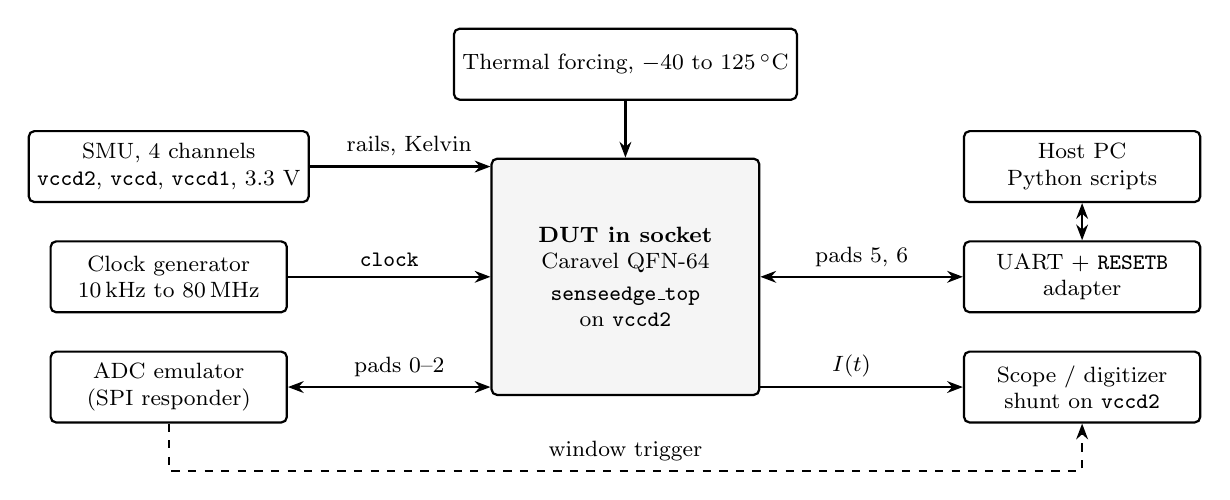
\begin{tikzpicture}[font=\footnotesize, x=1mm, y=1mm,
  b/.style={draw, thick, rounded corners=2pt, align=center, inner sep=3pt, minimum height=9mm},
  a/.style={-{Stealth[length=2mm]}, thick}, d/.style={{Stealth[length=2mm]}-{Stealth[length=2mm]}, thick}]
  \node[b, minimum width=34mm, minimum height=30mm, fill=black!4] (dut) at (0,0) {\textbf{DUT in socket}\\Caravel QFN-64\\[2pt]\texttt{senseedge\_top}\\on \texttt{vccd2}};
  \node[b, minimum width=30mm] (smu) at (-58, 14) {SMU, 4 channels\\\texttt{vccd2}, \texttt{vccd}, \texttt{vccd1}, 3.3 V};
  \node[b, minimum width=30mm] (clk) at (-58, 0) {Clock generator\\\SI{10}{\kilo\hertz} to \SI{80}{\mega\hertz}};
  \node[b, minimum width=30mm] (emu) at (-58, -14) {ADC emulator\\(SPI responder)};
  \node[b, minimum width=30mm] (host) at (58, 14) {Host PC\\Python scripts};
  \node[b, minimum width=30mm] (uart) at (58, 0) {UART + \texttt{RESETB}\\adapter};
  \node[b, minimum width=30mm] (scope) at (58, -14) {Scope / digitizer\\shunt on \texttt{vccd2}};
  \node[b, minimum width=34mm] (temp) at (0, 27) {Thermal forcing, $-40$ to \SI{125}{\celsius}};
  \draw[a] (smu.east) -- node[above, pos=0.55]{rails, Kelvin} (dut.west |- smu.east);
  \draw[a] (clk.east) -- node[above]{\texttt{clock}} (dut.west);
  \draw[d] (emu.east) -- node[above, pos=0.55]{pads 0--2} (dut.west |- emu.east);
  \draw[d] (uart.west) -- node[above]{pads 5, 6} (dut.east);
  \draw[a] (dut.east |- scope.west) -- node[above, pos=0.45]{$I(t)$} (scope.west);
  \draw[d] (host) -- (uart);
  \draw[a] (temp) -- (dut);
  \draw[a, dashed] (emu.south) -- ++(0,-6) -| node[above, pos=0.25]{window trigger} (scope.south);
\end{tikzpicture}
\caption{Characterization setup. The ADC emulator supplies known codes and
marks window boundaries; the host drives every sweep and stores raw data.}
\end{figure}

\subsection*{I1. Characterization board}
The sensor node ties the three \SI{1.8}{\volt} pins together, has a fixed
oscillator, and solders the ADC to the pads. None of the electrical tests
can run on it. A separate board is required:
\begin{itemize}
\item QFN-64 test socket, so that all 50 parts can be measured.
\item Separate Kelvin-sensed feeds for \texttt{vccd2} (macro), \texttt{vccd}
(management core), \texttt{vccd1} (pad controls and the user-side enables
of the isolation block; it must stay powered), and the \SI{3.3}{\volt}
rails. A shunt footprint in the \texttt{vccd2} feed with bulk decoupling
on the supply side only.
\item \SI{50}{\ohm} clock input to the \texttt{clock} pin. The harness
passes the external clock straight to the core at reset.
\item Header on pads 0--6, \texttt{RESETB}, the management GPIO, and the
flash pins. Pads 1--4 are also the housekeeping SPI used to program the
flash, so the header must give a programmer access to them.
\item Footprint for the real ADC and an analog input, selectable against
the emulator, for group D.
\end{itemize}

\subsection*{I2. Instruments}
\begin{itemize}
\item Four-channel source-measure unit, current resolution \SI{10}{\nano\ampere}
or better, digitizing at \SI{100}{kS/s} or better on the \texttt{vccd2} channel.
\item Clock generator, \SI{10}{\kilo\hertz} to \SI{80}{\mega\hertz}, with a
gated or burst mode and a \SI{10}{\mega\hertz} reference output.
\item Oscilloscope, \SI{500}{\mega\hertz}, with a differential probe for the shunt.
\item Thermal forcing for the socket, $-40$ to \SI{125}{\celsius}, with a
thermocouple at the package.
\item Low-distortion signal source locked to the clock generator's reference.
\item Reference vibration chain: IEPE accelerometer, 24-bit acquisition at
\SI{25.6}{kS/s} or more, tachometer, small shaker.
\end{itemize}

\subsection*{I3. ADC emulator}
An FPGA or a microcontroller with a deterministic SPI responder that
reproduces the MCP3201 frame (two sample clocks, null bit, twelve data
bits, LSB-first repeat). Requirements: serial clock to \SI{10}{\mega\hertz};
replay memory for at least \num{65536} codes; state advanced only by the
serial clock, so a paused chip resumes cleanly; a trigger output at the
64th sample of each window; codes loaded from the host.

\subsection*{I4. Firmware for the management core}
\begin{itemize}
\item \textbf{Monitor.} Peek, poke, and burst read over the hardware UART
(TX on pad 6, RX on pad 5). Pad 5 stays under management control; pads
0--4 are handed to the user area and the housekeeping SPI is disabled.
\item \textbf{Self-check.} After each decision flag: clear enable, read
the 32 bins and 8 features, compare a CRC with a table built from RTL
simulation, count mismatches, set enable. No UART traffic per window.
\item \textbf{Free run.} Chain enabled, nothing read; used for power.
\item \textbf{Software pipeline.} The same capture arithmetic, FFT,
features, and network in C, bit-exact to the netlist model, for test E1.
\item \textbf{Firmware classifier.} The 8--16--4 network on features read
from the chip, with weights in a table.
\end{itemize}
All register offsets are word offsets from \texttt{0x3000\_0000}. The
firmware in the repository does not address the chip correctly and is not
a starting point.

\subsection*{I5. Golden data}
The RTL is the golden model; the post-route netlist returns the same bins
and features from three power-up states. Vector sets, generated by
\texttt{proposal/src/run\_sims.py}:
\begin{description}[leftmargin=2.2em,style=nextline,itemsep=0pt]
\item[V1] Impulse records, one non-zero sample per window, stepping
through all \num{4096} codes. Every bin then equals the magnitude of that
sample, which reads the capture transfer out through the FFT.
\item[V2] One tone per bin, 0 to 31, at three amplitudes.
\item[V3] \num{4096} random three-tone records with noise and offset.
\item[V4] Corner cases: full-scale wrap, magnitude saturation, constant codes, alternating codes.
\item[V5] Recorded vibration: the testbed recordings of group F and the
CWRU set, resampled to the chip rate.
\end{description}

\subsection*{I6. Rehearsal}
The firmware, emulator model, and host scripts run first against the full
Caravel RTL in co-simulation and then against the user macro on an FPGA
behind the same pads. No script meets silicon untested.

\subsection*{I7. Data discipline}
Every record carries die number, board, firmware hash, script commit,
instrument, calibration date, and ambient temperature. Raw data are kept;
figures are generated by script from raw data. Dice are numbered on
arrival and never re-numbered.

\section{Tests}
\label{sec:tests}
Predictions in \pred{italics}. ``Pass'' in groups B and C means zero
mismatches in self-check.

\subsection*{Group A: incoming and bring-up \normalfont(all parts)}
{\small
\begin{longtable}{@{}L{0.8cm}L{3.3cm}L{6.6cm}L{4.3cm}@{}}
\toprule
ID & Test & Procedure & Acceptance and record\\
\midrule
\endhead
\tid{A1} & Continuity & Pin-to-rail resistance in the socket, unpowered & No shorts between rails\\
\tid{A2} & Rails, quiescent & Ramp each rail with current limit, clock held low & Currents per rail; \pred{microamperes on \texttt{vccd2}}\\
\tid{A3} & Housekeeping & Read the housekeeping ID over SPI before any firmware runs & Life sign independent of firmware\\
\tid{A4} & Boot & Program flash, release reset, UART banner & Boot at \SI{10}{\mega\hertz}\\
\tid{A5} & Pad handover & Configure pads 0--4 as user, 5--6 management; read pad states & Pads as configured\\
\tid{A6} & Register map & Read status; write and read back control, alarm, divider registers; time one read & Values match; read time sets the self-check divider\\
\tid{A7} & First window & Emulator sends a bin-8 tone; read bins and features & Bit-exact to RTL. \textbf{Gate G1}\\
\bottomrule
\end{longtable}}

\subsection*{Group B: functional correctness, bit-exact \normalfont(3 dice in full, all dice on V2)}
{\small
\begin{longtable}{@{}L{0.8cm}L{3.3cm}L{6.6cm}L{4.3cm}@{}}
\toprule
ID & Test & Procedure & Acceptance and record\\
\midrule
\endhead
\tid{B1} & Capture transfer & V1 at $D=4$, \SI{20}{\mega\hertz}; bin value against code & \pred{$|2(c-2048)+c_1|$ with wrap at $\pm1024$}; plot against the RTL curve\\
\tid{B2} & FFT & V2, V3, V4; at least \num{e5} windows & Zero mismatches against RTL\\
\tid{B3} & Features & Same runs; feature read-back & Zero mismatches; band map as predicted\\
\tid{B4} & Timing constants & Trigger at 64th sample; decision flag captured by a management timer; current signature as a second measure; $D=0$, 1, 4, 249 & \pred{729 clocks; window $2240\,(D+1)$, \num{2304} at $D=0$}; identical results at every $D$\\
\tid{B5} & Alarm and interrupt & Log class and confidence per window with the alarm pad and interrupt flag over \num{e4} windows & Pad and flag follow the alarm model applied to the logged sequence\\
\tid{B6} & Soak & Self-check on V3 for \num{e8} windows at nominal, and \num{e7} at $V_{\min}+\SI{50}{\milli\volt}$ & Zero errors; quote the \SI{95}{\percent} upper bound $3/N$\\
\tid{N1} & Network as fabricated & (a) Fixed records, 100 power cycles per die, 10 dice: log class and confidence. (b) Step each reachable weight, log the response. (c) Write the addresses above \texttt{0x74}; confirm no response & Documents the defect on silicon: repeatability of the power-up state within and across dice; \pred{22 responsive registers}\\
\bottomrule
\end{longtable}}

\subsection*{Group C: electrical characterization}
\texttt{vccd} and \texttt{vccd1} stay at \SI{1.8}{\volt} unless stated;
\texttt{vccd2} is the swept supply. Three dice receive every test at
four temperatures. At least 20 dice receive the reduced set of C9.
{\small
\begin{longtable}{@{}L{0.8cm}L{3.3cm}L{6.6cm}L{4.3cm}@{}}
\toprule
ID & Test & Procedure & Acceptance and record\\
\midrule
\endhead
\tid{C1} & Leakage & Clock stopped low and high; \texttt{vccd2} from 0.6 to \SI{1.95}{\volt}; each temperature & $I_{\mathrm{leak}}(V,T)$; \pred{\SI{0.7}{\micro\watt} at \SI{1.8}{\volt}, \SI{25}{\celsius}}\\
\tid{C2} & Power against frequency & Free run; $f_{\mathrm{clk}}$ from \SI{50}{\kilo\hertz} to the limit, 12 points; 6 supplies; modes: chain disabled, chain enabled & Fit $P=E_{\mathrm{clk}}(V)f+P_{\mathrm{leak}}$; \pred{$E_{\mathrm{clk}}=\SI{0.65}{\nano\joule}$ at \SI{1.8}{\volt}}; enabled minus disabled gives the activity share\\
\tid{C3} & Shmoo & Self-check, 256 windows per point; \texttt{vccd2} 1.95 to \SI{0.8}{\volt} in \SI{50}{\milli\volt}; $f_{\mathrm{clk}}$ 1 to \SI{80}{\mega\hertz}; boundary points repeated with 4096 windows & Pass map; \pred{\SI{42}{\mega\hertz} at \SI{1.8}{\volt}, \SI{25}{\celsius}}. Failures that persist at low frequency and worsen cold and at high supply are hold failures: log separately\\
\tid{C4} & Minimum-energy point & $D=0$, $f_{\mathrm{clk}}=36f_s$ for $f_s$ = 1, 2.29, 4, 8~kS/s; lower \texttt{vccd2} to failure; energy per window from the digitized current over 1000 windows & $E_{\mathrm{win}}(V)$ and $V_{\min}$ per rate; location of the minimum; \pred{\SI{1.5}{\micro\joule} at \SI{1.8}{\volt}}\\
\tid{C5} & Energy per classification & Charge on \texttt{vccd2} over 1000 triggered windows at three points: reset configuration; $D=0$ matched clock at nominal; the minimum of C4 & Headline numbers with uncertainty; \pred{\SI{0.36}{\milli\joule}, \SI{1.5}{\micro\joule}}\\
\tid{C6} & Phase-resolved energy & $f_{\mathrm{clk}}=\SI{100}{\kilo\hertz}$ so the pass lasts \SI{7.3}{\milli\second}; average the current over 1000 triggered passes; subtract the clock-only baseline & Energy of FFT, features, network, and acquisition; \pred{split close to 483 : 37 : 209 because the clock dominates}\\
\tid{C7} & Interface floor & Repeat the low-voltage edge of C3 with all three \SI{1.8}{\volt} rails swept together & Separates core failure from level mismatch at the domain boundary\\
\tid{C8} & Temperature & C1--C5 at $-40$, 25, 85, \SI{125}{\celsius} & Energy per classification against temperature for both clock policies\\
\tid{C9} & Die-to-die & At least 20 dice at \SI{25}{\celsius}: leakage and power at \SI{1.8}{\volt}; $f_{\max}$ at 1.6, 1.8, \SI{1.95}{\volt}; $V_{\min}$ at $D=0$, \SI{2.29}{kS/s}; V2 bit-exact & Histograms, mean and standard deviation, functional yield of 50; model-to-hardware table against Section~\ref{sec:pred}\\
\bottomrule
\end{longtable}}

\noindent\textbf{Harness limits to state in the paper.} The management
core shares the clock, so the measurable $f_{\max}$ is capped by the core
and its flash. If the macro still passes at that cap, report the cap and
the $V_{\min}(f)$ curve below it. A Wishbone access to a macro below its
working voltage never returns; the host must time out and pulse
\texttt{RESETB}.

\subsection*{Group D: signal chain with the real ADC and sensor}
{\small
\begin{longtable}{@{}L{0.8cm}L{3.3cm}L{6.6cm}L{4.3cm}@{}}
\toprule
ID & Test & Procedure & Acceptance and record\\
\midrule
\endhead
\tid{D1} & ADC and capture & Bin-centred sine into the ADC, source locked to the chip clock, 8 amplitudes; raise the serial clock until bins degrade & Bin magnitude against input; spur level; noise floor per bin; maximum usable sample rate at \SI{3.3}{\volt}\\
\tid{D2} & Acceleration response & Node and reference accelerometer on the shaker; stepped sine 5~Hz to \SI{3}{\kilo\hertz}; three sample rates & LSB per $g$ against frequency; noise floor in $g$; rejection of tones above half the sample rate\\
\tid{D3} & Feature fidelity & Shaker multi-tone and motor signals; reference signal resampled and passed through the bit-exact model & Chip feature against reference feature: scatter, error histogram per feature\\
\tid{D4} & Offset and orientation & Features with the sensing axis along and across gravity, before and after the offset remedy on the board & DC leakage into the high band, and its removal\\
\bottomrule
\end{longtable}}

\subsection*{Group E: system and baselines}
{\small
\begin{longtable}{@{}L{0.8cm}L{3.3cm}L{6.6cm}L{4.3cm}@{}}
\toprule
ID & Test & Procedure & Acceptance and record\\
\midrule
\endhead
\tid{E1} & Same-die software baseline & Software pipeline on the management core over V3; cycles from the core timer; energy from \texttt{vccd} minus its idle & Cycles and energy per classification, software against hardware, same die, same process, same vectors. Outputs must match bit for bit\\
\tid{E2} & Microcontroller baseline & The same C pipeline with its own ADC on a commercial low-power microcontroller, measured with the same instrument & One row of the comparison table that is measured, not quoted\\
\tid{E3} & Node power & Sensor node, every rail, at 1, 2.29, 4~kS/s continuous and at 1 and 10 classifications per second with the clock stopped between windows. Bursts are exactly \num{2304} clocks at $D=0$, aligned to the window, so each record is contiguous; the decision for a window appears in the next burst & Breakdown: sensor, ADC, macro, management core, oscillator, regulators, radio. One week on a stated cell, measured\\
\tid{E4} & Hybrid decision cost & Firmware classifier on chip features: cycles and energy per decision & Cost of the classifier as it runs on revision A\\
\bottomrule
\end{longtable}}

\subsection*{Group F: classification and deployment on physical faults}
{\small
\begin{longtable}{@{}L{0.8cm}L{3.3cm}L{6.6cm}L{4.3cm}@{}}
\toprule
ID & Test & Procedure & Acceptance and record\\
\midrule
\endhead
\tid{F1} & Testbed & Motor with variable-speed drive and load; bearing housing with exchangeable bearings; imbalance disc with measured masses; adjustable base for measured misalignment. Reference accelerometer beside the node, tachometer & Fault severities stated in physical units; photographs; drawing\\
\tid{F2} & Dataset & Healthy and three faults; two severities; three speeds; two loads; five reassemblies on different days; 2~min per session; chip features and reference signal recorded together & About 210 sessions. The session is the statistical unit, never the window\\
\tid{F3} & Model ladder & On identical data: (i) chip features, INT8 8--16--4; (ii) chip features, floating point; (iii) designed bands recomputed from chip bins; (iv) 1024-point reference features with a stronger model; (v) RMS threshold. Leave-one-reassembly-out and leave-one-speed-out & Accuracy with \SI{95}{\percent} interval from a session bootstrap; confusion matrix; what the 64-point front end, the shifted bands, and INT8 each cost\\
\tid{F4} & Sample-rate policy & Fixed rate against a rate tied to shaft speed so that the shaft line sits in bin 2 or 3 & Accuracy against policy; the shaft line is otherwise lost in bin 1\\
\tid{F5} & Live run & Node classifies in real time for at least two weeks; faults introduced on a schedule unknown to the classifier; alarm depth swept offline on the log & Detection delay, false alarms per week against depth, drift against temperature, one firmware model update with before and after\\
\tid{F6} & Second machine & A pump or fan; retrain; repeat F3 (i) and (iv) & Retargeting cost in data and accuracy\\
\tid{F7} & Public benchmark on silicon & CWRU records replayed through the emulator; chip features; ladder (i), (ii) & A number others can reproduce, measured on the chip\\
\bottomrule
\end{longtable}}

\section{What each test puts in the paper}
{\small
\begin{longtable}{@{}L{6.4cm}L{2.2cm}L{6.4cm}@{}}
\toprule
Figure or table & From & Note\\
\midrule
\endhead
Chip micrograph with macro outline & --- & Decapsulate one part or obtain a bare die; a layout plot does not replace it\\
Measurement setup, photo and diagram & I1--I3 & \\
Capture transfer and spectrum, silicon against RTL & B1, B2 & Bit-exact statement with window count\\
Shmoo, three temperatures & C3, C8 & Hold-type failures marked\\
Power against frequency; energy per clock against supply & C2 & With the fit and the prediction\\
Energy per classification against supply, both clock policies & C4, C5 & The headline figure\\
Phase-resolved current of one pass & C6 & Replaces the ``per-block enable'' pie\\
Leakage and energy against temperature & C1, C8 & \\
Die-to-die histograms & C9 & $N\ge20$\\
Model-to-hardware correlation table & C9 & Predictions of Section~\ref{sec:pred}\\
Chain response and noise floor & D1, D2 & In physical units\\
Hardware against software on the same die & E1 & Cycles and energy ratio\\
Node power breakdown; measured cell life & E3 & \\
Confusion matrix; model ladder & F3 & With intervals\\
Deployment timeline, false alarms against depth & F5 & \\
Comparison table & C5, E2, F3 & Energy with stated definition; one measured baseline row\\
\bottomrule
\end{longtable}}

\section{Reporting rules}
\begin{itemize}
\item Every number carries supply, clock, divider, temperature, and the
number of dice. Energy per classification always states what a
classification includes.
\item Uncertainty is stated: instrument accuracy, shunt tolerance, and
repeatability over five repeats. Die-to-die spread is reported
separately from measurement uncertainty.
\item Zero observed errors is reported as an upper bound, $3/N$ at
\SI{95}{\percent}.
\item Accuracy is reported with an interval, on data split by session,
with the split written down before the data are taken.
\item The defects are reported: the weight decoder, the two signedness
errors, the feature alignment, and the capture slice, with the silicon
evidence of N1, B1, and B3.
\item Scripts, raw data, vectors, and firmware are released with the paper.
\end{itemize}

\section{Schedule and gates}
{\small
\begin{longtable}{@{}L{2.6cm}L{8.4cm}L{4.0cm}@{}}
\toprule
When & Work & Gate\\
\midrule
\endhead
Now & Decide framing and revision B. Order socket, design characterization board. Revise the node board (Appendix~\ref{app:board}) before fabrication & \textbf{G0}: claims fixed\\
Before silicon & Board, emulator, firmware, host scripts; rehearsal in co-simulation and on FPGA; vector sets; testbed and reference chain built; F2 split written down & Rehearsal passes end to end\\
Weeks 1--2 & A on all parts; B on three dice & \textbf{G1}: first window bit-exact. \textbf{G2}: B2, B3 clean\\
Weeks 2--4 & C1--C7 on three dice at \SI{25}{\celsius}; E1 & Energy headline fixed\\
Weeks 4--6 & C8 temperature; C9 twenty dice; B6 soak; N1 & \textbf{G3}: silicon section complete for CICC\\
Weeks 3--8 & D on the node; F1--F4 dataset and ladder; E2--E4 & Accuracy with intervals\\
Weeks 6--12 & F5 live run; F6, F7 & \textbf{G4}: deployment section complete for the journal version\\
\bottomrule
\end{longtable}}

\section{Risks specific to this chip}
\begin{itemize}
\item \textbf{Hold margin.} \SI{0.06}{\nano\second} at the fast corner.
A die that fails at every frequency when cold or at high supply is a hold
failure. Lower supply and higher temperature are the workaround; record
which dice need it.
\item \textbf{Port-path timing.} The reset and Wishbone input paths
violate under the assumed arrival times. Symptom: wrong register writes
or a chain that does not start cleanly after reset. A6 and A7 catch it.
\item \textbf{Clock cap.} The management core may fail before the macro.
Report it as a harness limit.
\item \textbf{Domain boundary.} With \texttt{vccd2} below about
\SI{1}{\volt} the macro's outputs may no longer switch the
\SI{1.8}{\volt} receivers. C7 distinguishes this from core failure.
\item \textbf{Flash access.} Programming needs pads 1--4, which the node
wires to the ADC and LEDs. Without a header the flash cannot be
reprogrammed in place.
\item \textbf{Leakage at temperature.} It may dominate the slow-clock
mode. If it does, report it; it is a result.
\end{itemize}

\appendix
\section{Changes to the node board before it is fabricated}
\label{app:board}
The node has not been assembled, so these cost a layout revision and not
a rework.
\begin{enumerate}
\item Feed \texttt{vccd2}, \texttt{vccd1}, and \texttt{vccd} through
separate jumpers with shunt footprints.
\item Make the clock controllable: oscillator through a jumper, a
footprint for an external input, and the oscillator enable on a radio
GPIO. A clock from the radio module at 36 times the sample rate, with the
divider at zero, is the low-power mode.
\item Put a series jumper in the ADC data line and bring pads 0--4,
\texttt{RESETB}, and the UART to a header, for the emulator and for flash
programming.
\item Centre the sensor at mid-scale: AC coupling into a mid-supply bias,
or an offset trim. Set the sensor bandwidth from the chosen sample rate;
with the fitted \SI{3.3}{\nano\farad} the bandwidth is
\SI{1.5}{\kilo\hertz}, which aliases at every rate below
\SI{3}{kS/s}.
\item Swap the UART pins on the radio side: the harness transmits on
pad 6 and receives on pad 5.
\item Check the \SI{1.8}{\volt} regulator rating against C2. The macro
alone is predicted at \SI{7}{\milli\ampere} at \SI{20}{\mega\hertz}.
\item Populate the \SI{20}{\mega\hertz} oscillator and one accelerometer
part; the BOM file lists a crystal and a different sensor.
\end{enumerate}

\section{Revision B, if the journal version is to claim the on-chip classifier}
The same suite applies with three additions: weight read-back makes the
network bit-exact test direct (B-group, all 212 registers); a
register-map model update replaces the firmware-table update in F5; and
clock gating adds a third clock policy to C4 and C5. Before a shuttle
slot is committed the corrected RTL runs on the FPGA of I6 behind the
node's front end, through groups B, D, and F.

\end{document}
